  \documentclass[a4paper, titlepage]{report}
\usepackage[utf8]{inputenc}
\usepackage[T1]{fontenc}
\usepackage[french]{babel}

\usepackage{graphicx} 


\usepackage{lmodern} % Pour changer le pack de police
\usepackage[vlined, longend]{algorithm2e}
\usepackage{multicol}
\usepackage[a4paper, top=2cm, bottom=2cm, left=2cm, right=2cm]{geometry}


\usepackage{wrapfig}
 


\setlength{\algomargin}{0em}
\SetKwRepeat{Repeat}{Do}{While}
\SetKwIF{If}{ElseIf}{Else}{If}{then}{Else if}{Else}{EndIf}
\SetKwFor{For}{For}{do}{Done}
\SetKwFor{While}{While}{do}{Done}

\providecommand{\SetAlgoLined}{\SetLine}
\providecommand{\DontPrintSemicolon}{\dontprintsemicolon}

\SetKwBlock{Begin}{Begin}{End}

\SetKw{KwFrom}{from }
\SetKw{KwBy}{by }
\DontPrintSemicolon	% do not print the ';' symbol
\newcommand{\TRUE}{\textit{TRUE} }
\newcommand{\FALSE}{\textit{FALSE} }
\newcommand{\AND}{\textit{AND} }
\newcommand{\OR}{\textit{OR} }
\newcommand{\NULL}{\textit{NULL} }

\newcommand{\NewWhile}{\SetKwBlock{While}{while}{}}
\newcommand{\NormalWhile}{\SetKwBlock{While}{while}{Done}}

\setcounter{secnumdepth}{5}
\setcounter{tocdepth}{5}

\newenvironment{lexicon}{\noindent \hspace{1.2em} {\bf \underline{Lexicon}} \\~\\}{ ~\\ }
\newenvironment{algo}{\noindent \hspace{1.2em} {\bf \underline{Algorithm}} \\~\\ \begin{algorithm}[H] \SetAlgoLined }{\end{algorithm}  ~\\}

\usepackage{listings}
\lstset{ 
language=java
}

\title{LO43 
     Flotte de véhicules autonomes}
\author{Buri Theo florian Lacour} 
\date{Hiver 2013}

\makeatletter
\def\clap#1{\hbox to 0pt{\hss #1\hss}}%
\def\ligne#1{%
\hbox to \hsize{%
\vbox{\centering #1}}}%
\def\haut#1#2#3{%
\hbox to \hsize{%
\rlap{\vtop{\raggedright #1}}%
\hss
\clap{\vtop{\centering #2}}%
\hss
\llap{\vtop{\raggedleft #3}}}}%
\def\bas#1#2#3{%
\hbox to \hsize{%
\rlap{\vbox{\raggedright #1}}%
\hss
\clap{\vbox{\centering #2}}%
\hss
\llap{\vbox{\raggedleft #3}}}}%
\def\maketitle{%
\thispagestyle{empty}\vbox to \vsize{%
\haut{}{\@blurb}{}
\vfill
\vspace{1cm}
\begin{flushleft}
\usefont{OT1}{ptm}{m}{n}
\huge \@title
\end{flushleft}
\par
\hrule height 4pt
\par
\begin{flushright}
\usefont{OT1}{phv}{m}{n}
\Large \@author
\par
\end{flushright}
\vspace{1cm}
\vfill
\vfill
\bas{}{\@location, \@date}{}
}%
\cleardoublepage
}
\def\date#1{\def\@date{#1}}
\def\author#1{\def\@author{#1}}
\def\title#1{\def\@title{#1}}
\def\location#1{\def\@location{#1}}
\def\blurb#1{\def\@blurb{#1}}
\date{Décembre 2014}
\author{}
\title{}
\makeatother
\title{LO43 Flotte de véhicule autonomes}
\author{Buri Theo Florian Lacour}
\location{Belfort}
\blurb{%
Université de technologie de Belfort-Montbéliard
}% 

\usepackage{array}


\begin{document}


\maketitle
\tableofcontents
\newpage
\chapter*{Introduction}
\addcontentsline{toc}{chapter}{Introduction}
\hspace{0.5cm}Dans le cadre de  l'UV LO43 " Bases fondamentales de la programmation orientée objet", il nous a été demandé de réaliser un projet de groupe, afin de mettre en pratique les connaissances acquises lors des cours et TDs du semestre.
\\
Trois sujet nous on été présentés. Nous avons fait le choix de traiter le sujet de la "Flotte de véhicules autonomes", et ceci pour plusieurs raisons :
\begin{itemize}
  \item (A TROUVER)
  \item N'étant que deux, sur un maximum de quatre étudiants par groupe autorisés, les autres sujets ne nous ont pas parus réalisables en temps et en heures et sans bugs majeurs...
  \item (A TROUVER)
\end{itemize}
Nous présenterons tout d'abord le sujet, ses contraintes, et les libertés prises par rapport à celles-ci. Par la suite, nous parlerons des différents diagrammes UML, et les expliquerons. Enfin, nous terminerons par l'implémentation en Java et l'interface graphique.


\setcounter{chapter}{1}
\setcounter{section}{1}
\part{ Présentation du sujet}
\section{Objectif}
 Le programme à réaliser consistait en la modélisation d'une flotte de véhicules évoluant dans une infrastructure de circulation partagée. Pour cela, il a tout d'abord fallu modéliser la partie calculatoire à l'aide du langage UML, puis ensuite l'implémenter en Java et lui donner une interface graphique
\section{Reformulation du sujet}
\subsection{Plateau}
Le plateau donné par le sujet est le suivant :
\vspace{0.5cm}

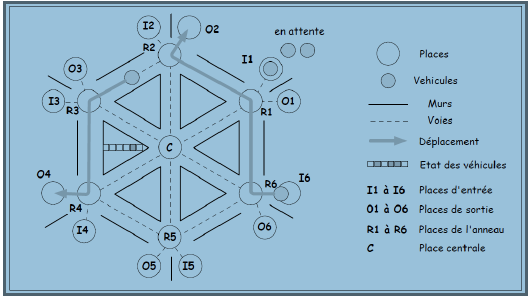
\includegraphics[]{Images/Plateau}
\vspace{0.5cm}
\\
Chaque place, exceptée celle du centre, est rattachée à une place de départ et une place de sortie. Les voitures disposant d'un passager partent depuis une place d'entrée (que celui-ci leur donne) et, à la fin de celle-ci, rejoignent une place de sortie (même chose).\\
La place centrale n'est utilisée que lors d'un trajet reliant deux places opposées...
\subsection{Passagerss et contrôleur}
Chaque passager doit être transporté d'une place à une autre. Pour ce faire, ils envoient une requête au module qui se charge du contrôle du plateau : le contrôleur. Par la suite, celui-ci assignera cette mission à un des véhicules de sa flotte (sous la forme d'un passager, ayant un départ et une arrivée). Celui-ci calculera ensuite le trajet qu'il suivra pour la mener à bien.\\
C'est alors le véhicule qui décide de partir : pour cela il doit envoyer une requête au contrôleur pour savoir si son chemin est déjà réservé. Si ce n'est pas le cas, le contrôleur l'autorise, et le véhicule part. La requête se fait sous la forme d'une Request Map, constituée de booléens indiquant l'intention du véhicule de réserver une place ou non.\\
Pour exemple, lorsqu'une voiture désire aller de la place I1 à O2, elle aura besoin de réserver I1, R1, R2 et O2. La Request Map seras alors la suivante :
\vspace{0.5cm}

\begin{tabular}{|l|l|l|l|l|l|l|l|l|l|l|l|l|l|l|l|l|l|l|l|}

\hline
  I1 & I2 & I3 & I4 & I5 & I6 & R1 & R2 & R3 & R4 & R5 & R6 & O1 & O2 & O3 & O4 & O5 & O6 & C \\
  \hline
   T & F & F & F & F & F & T & T & F & F & F & F & F & T & F & F & F & F & F\\
 \hline

\end{tabular}\\
\vspace{0.25cm}\\
Afin d'éviter toute erreur lors de la réservation, nous avons défini la priorité des places qui suit:
\begin{center}
I1<I2<I3<I4<I5<I6<R1<R2<R3<R4<R5<R6<O1<O2<O3<O4<O5<O6<C
\end{center}
Ceci permettra d'éviter que deux véhicules tentent de réserver la même place à deux moments différents, et que le contrôleur les valide...

\subsection{Contraintes et libertés prises sur le sujet}


S'ajoutent alors quelques contraintes, qui régissent le programme :
\begin{itemize}
  \item Les véhicules ne peuvent utiliser la place centrale qu'à la seule condition qu'ils doivent se rendre à la place en face de la leur.
  \item Une place ou une route (reliant deux places) ne peut être utilisée que par un seul et unique véhicule.
  \item Un véhicule qui souhaite emprunter un chemin occupé doit attendre que celui-ci se libère.
\end{itemize}
\vspace{0.25cm}
Ainsi, par rapport à ces différentes consignes, nous avons choisi de prendre certaines libertés :
\vspace{0.25cm}
\begin{itemize}
  \item Un véhicule ne peut pas contourner une place occupée pour mener sa mission à bien.
  \item 
\end{itemize}
\setcounter{chapter}{1}
\setcounter{section}{1}
\part{Conception UML}
%non de chapitre a changer

\chapter{Les Diagramme UML}
\section{Diagramme des cas d'utilisation (annexe A)}
\hspace{0.5cm} Le diagramme des cas d'utilisation permet de représenter les actions que l'utilisateur peut faire. Dans notre projet, en lançant le programme, l'utilisateur a plusieurs solutions :
\begin{itemize}
\item Voir les crédits (c'est à dire les auteurs du programme, nous)
\item Choisir de jouer en mode manuel, dans ce cas il devras par la suite choisir lui-même les missions attribuées aux véhicules.
\item Jouer en simulation, dans ce mode toutes les requête sont générées par le programme : l'utilisateur se contente de regarde la simulation s'opérer.
\item Avoir accès aux options : une fois dans ce menu, il peut choisir de changer la rapidité des voitures.
\end{itemize}
Nous avons choisi de diviser l'utilisateur principal en deux autres : un utilisateur qui utiliserait le mode manuel, et un autre qui utiliserait le mode automatique. Ceci étant dû au fait que l'utilisateur en mode manuel pourra accéder à des fonctions interdites au mode automatique (la création d'un passager).\\
En outre, une fois sur l'écran de "jeu" (où se déplacent les véhicules), l'utilisateur (et quel que soit son mode) pourra mettre la simulation en pause et, si nécessaire, réinitialiser celle-ci. 
\section{Diagramme de séquence(annexe B)}
\hspace{0.5cm} Le diagramme de séquence permet de représenter les interactions entre les différentes classes selon un ordre chronologique.
\section{Diagramme de classes(annexe C)}
\hspace{0.5cm} Nous verrons en détail, une description de chaque classe.
\chapter{Description des classes}
\section{Classe BoiteAuxLettre}
     
      Il s'agit de la classe recevant toute les requêtes, qu'elles soient envoyées depuis la partie graphique (c'est à dire des requêtes pour la création d'une nouvelle mission, et donc d'un nouveau passager), ou du modèle. Il y a 4 requêtes différentes, stockées chacunes dans une liste différente:
      \begin{wrapfigure}[15]{l}{5.5cm}
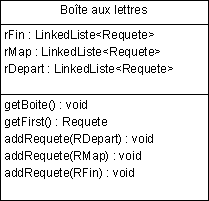
\includegraphics[scale=1]{Images/BoiteAuxLettre.PNG}
\end{wrapfigure}   
      \begin{itemize}
      \item Une liste de requêtes de départ : cette liste contient toutes les demandes de trajet. Ces trajet peuvent être demandés soit par l'utilisateur, soit générés par le modèle.
      \item Une liste de requêtes de trajet : ce sont les requêtes qu'envoient chacun des véhicules ayant un passager pour demander au contrôleur la permission d'utiliser un chemin (la réponse n'est positive que si le chemin concerné est libre)...
      \item Une liste de requêtes de fin de trajet : ce sont les requête qu'envoient les véhicules lorsqu'ils ont mené leur mission à bien (et donc qu'ils sont arrivés à leur place d'arrivée). Elles permettent alors de libérer le véhicule.
      \item Enfin, une liste de requêtes de libération de ressources : ces requêtes sont envoyées par les véhicules lorsqu'il n'ont plus besoin d'une place (lorsqu'ils sont déjà passés de dessus). Le contrôleur peut alors considérer ces places comme disponibles.
      \end{itemize}

\section{Les classes Requêtes}

Etant donné que le but de chaque requête a été explicité ci-dessus, et que la structure de celles-ci ne présente pas d'intérêt particulier, nous nous intéresserons à leurs caractéristiques générales. \\
Chaque type de requêtes a sa propre liste, contenue dans la boîte aux lettres. Un requête, une fois traitée, est immédiatement détruite. Enfin,à chaque liste de requêtes est attribuée une priorité, afin que le contrôleur traite les requêtes les plus importantes en premier.
\section{La classes Contrôleur}

Il s'agit de la classe principale : c'est elle qui s'occupe de gérer les déplacements des différents véhicules sur la carte. Le contrôleur a directement accès à la boîte aux lettres, et donc aux requêtes qu'elle contient.\\
C'est également lui qui possède la "carte" (ici, une HashMap) des différentes places du réseau routier : il est le seul à agir dessus.
La méthode traiteRequete() se charge de traiter les requêtes selon leur priorité :\\
 \begin{itemize}
      \item Les requêtes de fin de trajet sont prioritaires sur toutes les autres : rendre un véhicule à nouveau disponible signifie le débarquement d'un passager, et donc la capacité d'en accepter de nouveaux.
      \item Les requêtes de libération de ressources arrivent en second. En effet, rendre une place disponible le plus vite possible est prioritaire pour pouvoir valider les trajets d'autres véhicules.
      \item Viennent ensuite les requêtes de départ, permettant aux passagers d'être pris en charge plus vite que les requêtes de trajet, bien plus nombreuses.
      \item Les requêtes de trajet sont les moins prioritaires, notamment en raison de le nombre : en effet, elles sont générées à intervalle régulier par les véhicules, jusqu'à ce qu'ils aient pu emprunter le chemin qu'ils désirent.
      \end{itemize}

Par la suite, et en fonction des requêtes qu'il reçoit, le contrôleur a plusieurs tâches. Il peut libérer un véhicule en fin de trajet, en réserver un autre et lui attribuer un passager. Enfin, il valide (ou non) les chemins demandés par les véhicules, et se charge ensuite de réserver les ressources correspondantes.
%  les annexes
\appendix
%diagrame cas d'utilisation
\chapter*{Annexe A}
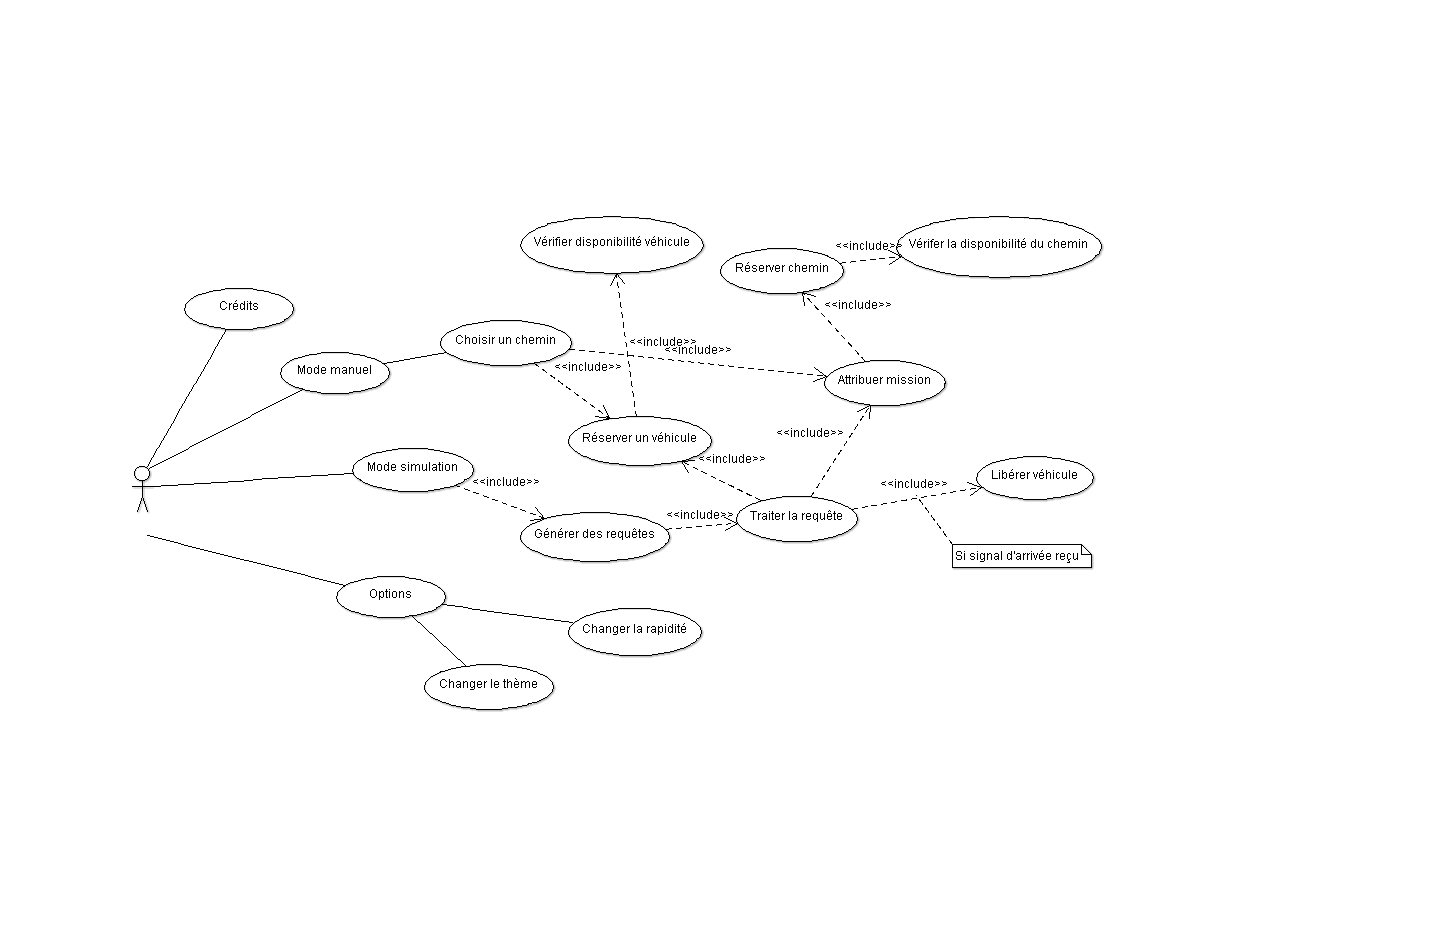
\includegraphics[width=455px, height=190px]{Images/CasUtilisation.PNG}
%diagrame de sequence
\chapter*{Annexe B}
\end{document}